% F6: M4's evaluation-time disruption harness -- where each of the three
% disruption kinds (dropout, churn, spike) intercepts the per-step
% control loop that Alg. 1/2's trained, FROZEN policy runs at eval time.
% Standalone-compilable; \input{}/\includegraphics{} into the paper body.
% Mirrors fig1_gat_ctde_fl_architecture.tex's style conventions (box/
% arrow styles, font, palette) so the two read as one visual family.
\documentclass[tikz,border=2pt]{standalone}
\usepackage{amsmath}
\usetikzlibrary{arrows.meta,positioning,fit,backgrounds}

\begin{document}
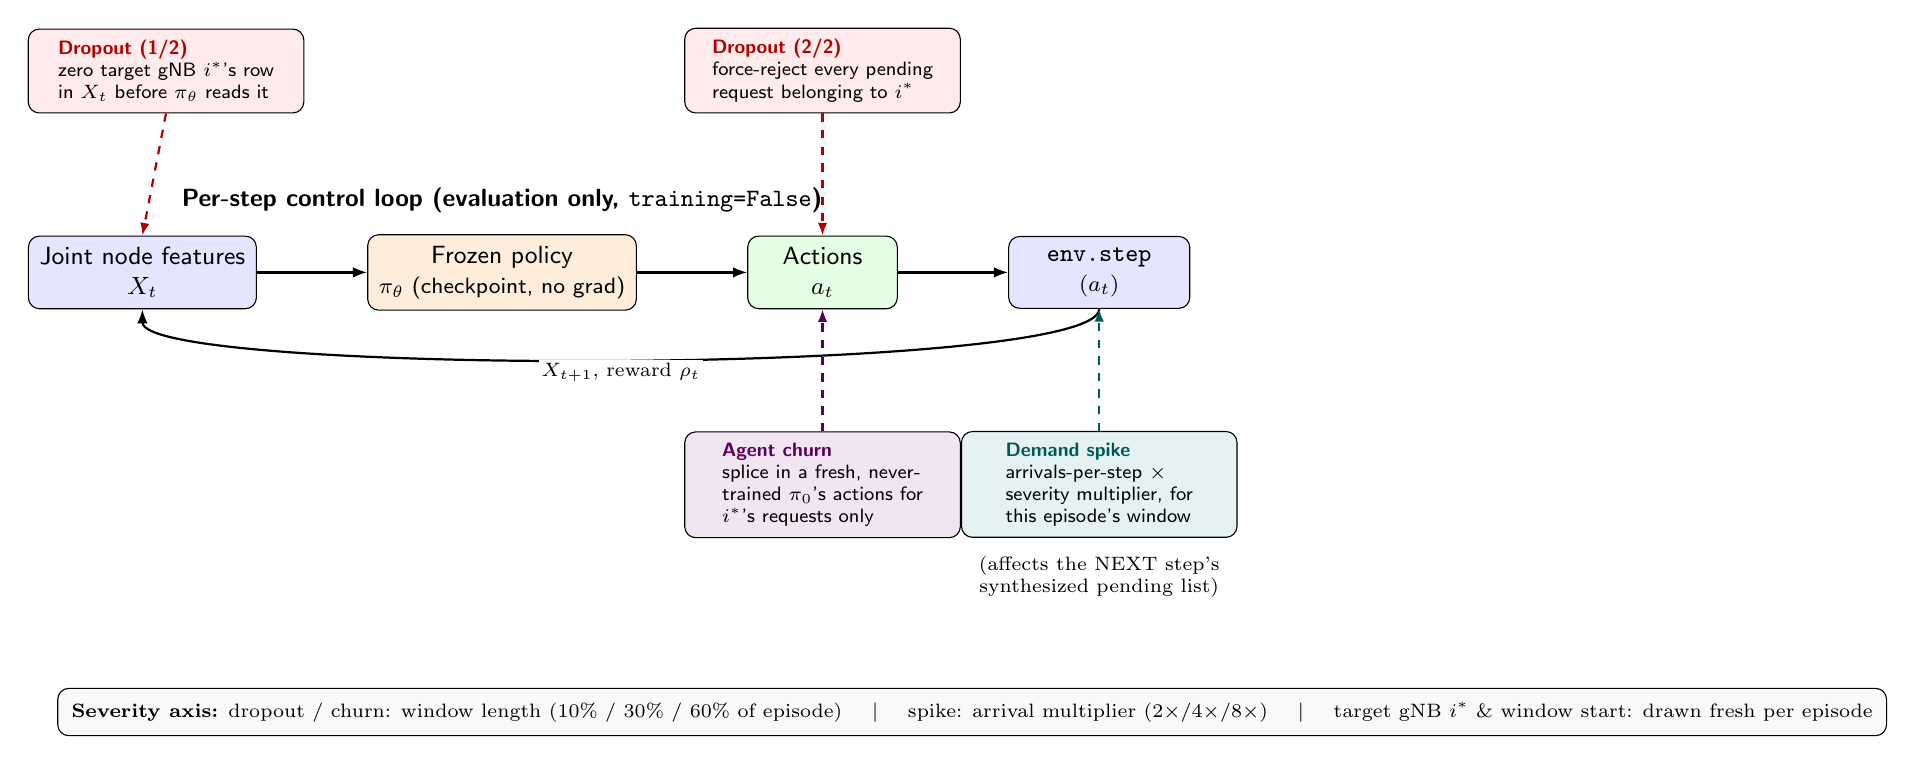
\begin{tikzpicture}[
  font=\sffamily\small,
  box/.style={draw, rounded corners, minimum height=0.9cm, align=center, inner sep=4pt},
  state/.style={box, fill=blue!10, minimum width=2.1cm},
  policy/.style={box, fill=orange!14, minimum width=2.5cm},
  envbox/.style={box, fill=blue!10, minimum width=2.3cm},
  actionbox/.style={box, fill=green!10, minimum width=1.9cm, minimum height=0.75cm},
  disrupt/.style={draw, rounded corners, fill=red!8, align=left, font=\sffamily\scriptsize, inner sep=4pt, minimum width=3.5cm},
  churnbox/.style={draw, rounded corners, fill=violet!10, align=left, font=\sffamily\scriptsize, inner sep=4pt, minimum width=3.5cm},
  spikebox/.style={draw, rounded corners, fill=teal!10, align=left, font=\sffamily\scriptsize, inner sep=4pt, minimum width=3.5cm},
  arrow/.style={-{Latex[length=1.8mm]}, thick},
  injectarrow/.style={-{Latex[length=1.6mm]}, thick, dashed},
]

% ===== Main per-step control loop (left to right) =====
\node[state] (x1) at (0,0) {Joint node features\\$X_t$};
\node[policy, right=1.4cm of x1] (pol) {Frozen policy\\\footnotesize $\pi_\theta$ (checkpoint, no grad)};
\node[actionbox, right=1.4cm of pol] (act) {Actions\\$a_t$};
\node[envbox, right=1.4cm of act] (env) {\texttt{env.step}\\\footnotesize$(a_t)$};

\draw[arrow] (x1) -- (pol);
\draw[arrow] (pol) -- (act);
\draw[arrow] (act) -- (env);

% Loop back to next step (shallow dip, stays clear of the legend below)
\draw[arrow] (env.south) .. controls +(0,-0.85) and +(0,-0.85) .. (x1.south)
  node[midway, below, font=\scriptsize, fill=white, inner sep=1pt] {$X_{t+1}$, reward $\rho_t$};

\node[font=\sffamily\bfseries\small, above=0.15cm of pol, xshift=0cm] {Per-step control loop (evaluation only, \texttt{training=False})};

% ===== Dropout: two injection points =====
\node[disrupt, above=1.55cm of x1, xshift=0.3cm] (drop1)
  {\textbf{\color{red!70!black}Dropout (1/2)}\\zero target gNB $i^*$'s row\\in $X_t$ before $\pi_\theta$ reads it};
\draw[injectarrow, red!70!black] (drop1.south) -- (x1.north);

\node[disrupt, above=1.55cm of act, xshift=0cm] (drop2)
  {\textbf{\color{red!70!black}Dropout (2/2)}\\force-reject every pending\\request belonging to $i^*$};
\draw[injectarrow, red!70!black] (drop2.south) -- (act.north);

% ===== Churn: one injection point, between policy output and dropout's forced-reject =====
\node[churnbox, below=1.55cm of act] (churn)
  {\textbf{\color{violet!70!black}Agent churn}\\splice in a fresh, never-\\trained $\pi_0$'s actions for\\$i^*$'s requests only};
\draw[injectarrow, violet!70!black] (churn.north) -- (act.south);

% ===== Spike: affects arrivals fed into env.step's OWN synthesis of step t+1's pending list =====
\node[spikebox, below=1.55cm of env] (spike)
  {\textbf{\color{teal!70!black}Demand spike}\\arrivals-per-step $\times$\\severity multiplier, for\\this episode's window};
\draw[injectarrow, teal!70!black] (spike.north) -- (env.south);

\node[font=\scriptsize, align=center, below=0.1cm of spike] {(affects the NEXT step's\\synthesized pending list)};

% ===== Severity legend =====
\node[draw, rounded corners, fill=gray!5, font=\scriptsize, align=left, inner sep=5pt,
      below=1.9cm of churn, xshift=1.9cm] (legend)
  {\textbf{Severity axis:} dropout / churn: window length (10\% / 30\% / 60\% of episode) $\quad\vert\quad$
   spike: arrival multiplier (2$\times$/4$\times$/8$\times$) $\quad\vert\quad$
   target gNB $i^*$ \& window start: drawn fresh per episode};

\end{tikzpicture}
\end{document}
